\section{Memoria Virtuale}
La \textbf{memoria virtuale} è una tecnica che consente a un sistema operativo di far sembrare che ogni processo abbia a disposizione un ampio spazio di memoria continuo e privato, anche se la memoria fisica (RAM) è limitata. In pratica, La memoria virtuale separa lo spazio di memoria logico (visto dal programma) da quello fisico. Inoltre, quando non c'è abbastanza memoria disponibile, parte dei dati può essere temporaneamente spostata su disco, in un'apposita area detta di swap. I componenti principali di una memoria virtuale sono:
\begin{itemize}
    \item \textbf{Spazio di indirizzamento virtuale}: \MakeUppercase{è} l'insieme degli indirizzi visti da un processo e viene suddiviso in pagine (solitamente di 4 KB ciascuna).
    \item \textbf{Memoria fisica}: Divisa in frame, della stessa dimensione delle pagine, ospita le pagine virtuali attualmente in uso.
    \item \textbf{Tabella delle pagine}: Mappa ogni pagina virtuale al corrispondente frame fisico (se presente). Contiene anche bit di validità, bit di accesso/scrittura, e altri flag.
    \item \textbf{Memory Management Unit (MMU)}: Hardware che effettua la traduzione automatica da indirizzo virtuale a fisico.
    \item \textbf{Translation Lookaside Buffer (TLB)}: Piccola cache specializzata per la tabella delle pagine. Serve a velocizzare la traduzione virtuale-fisica evitando accessi ripetuti alla page table.
    \item \textbf{Spazio di swap (su disco)}: Contiene le pagine che non stanno nella RAM. Quando serve una pagina assente in RAM (page fault), viene caricata da qui.
\end{itemize}

\subsection{Traduzione degli indirizzi}
Per poter accedere a una qualsiasi locazione, indipendentemente da dove essa sia situata (cache o RAM), il processore genera un indirizzo logico, il quale verrà poi opportunamente tradotto in un indirizzo fisico. L'indirizzo logico, è concettualmente costituito da due parti: la prima è l'identificativo di pagina, la seconda è lo spiazzamento (offset) nella pagina. A seconda della struttura della memoria virtuale (dimensione e numero delle pagine), il numero di bit richiesti per codificare i due campi può variare. Se un processo cerca di fare riferimento a un dato che fa parte di un blocco residente (cioè già caricato in memoria centrale), una struttura hardware effettua la traduzione dell'indirizzo logico in fisico, utilizzando delle opportune tabelle caricate dal sistema operativo. Un processo che invece tenta di fare riferimento a un blocco non residente, genera un'eccezione e viene sospeso, sarà poi compito del sistema operativo gestire il recupero del dato dalla memoria di massa. Il processo di traduzione avviene grazie a una tabella delle pagine mantenuta nella memoria centrale dal processore, la quale, per ogni pagina virtuale riporta l'identificativo della pagina fisica nella quale il SO l'ha allocata. Questa allocazione è dinamica, ovvero la pagina logica può essere posta in punti diversi della memoria principale in seguito a successive operazioni di allocazione e deallocazione. Un primo processo di traduzione avviene tramite le seguenti fasi [\ref{fig:traduzione}].
\begin{enumerate}
    \item La porzione di identificativo della pagine viene prelevata dall'indirizzo virtuale.
    \item L'identificativo viene sommato al puntatore alla tabella delle pagine, in modo da ricavare l'indirizzo della pagina fisica in cui il dato è allocato.
    \item L'indirizzo base ottenuto al punto precedente viene sommato con l'offset, prelevato dalla seconda parte dell'indirizzo logico.
\end{enumerate}

\begin{figure}[!h]
    \centering
    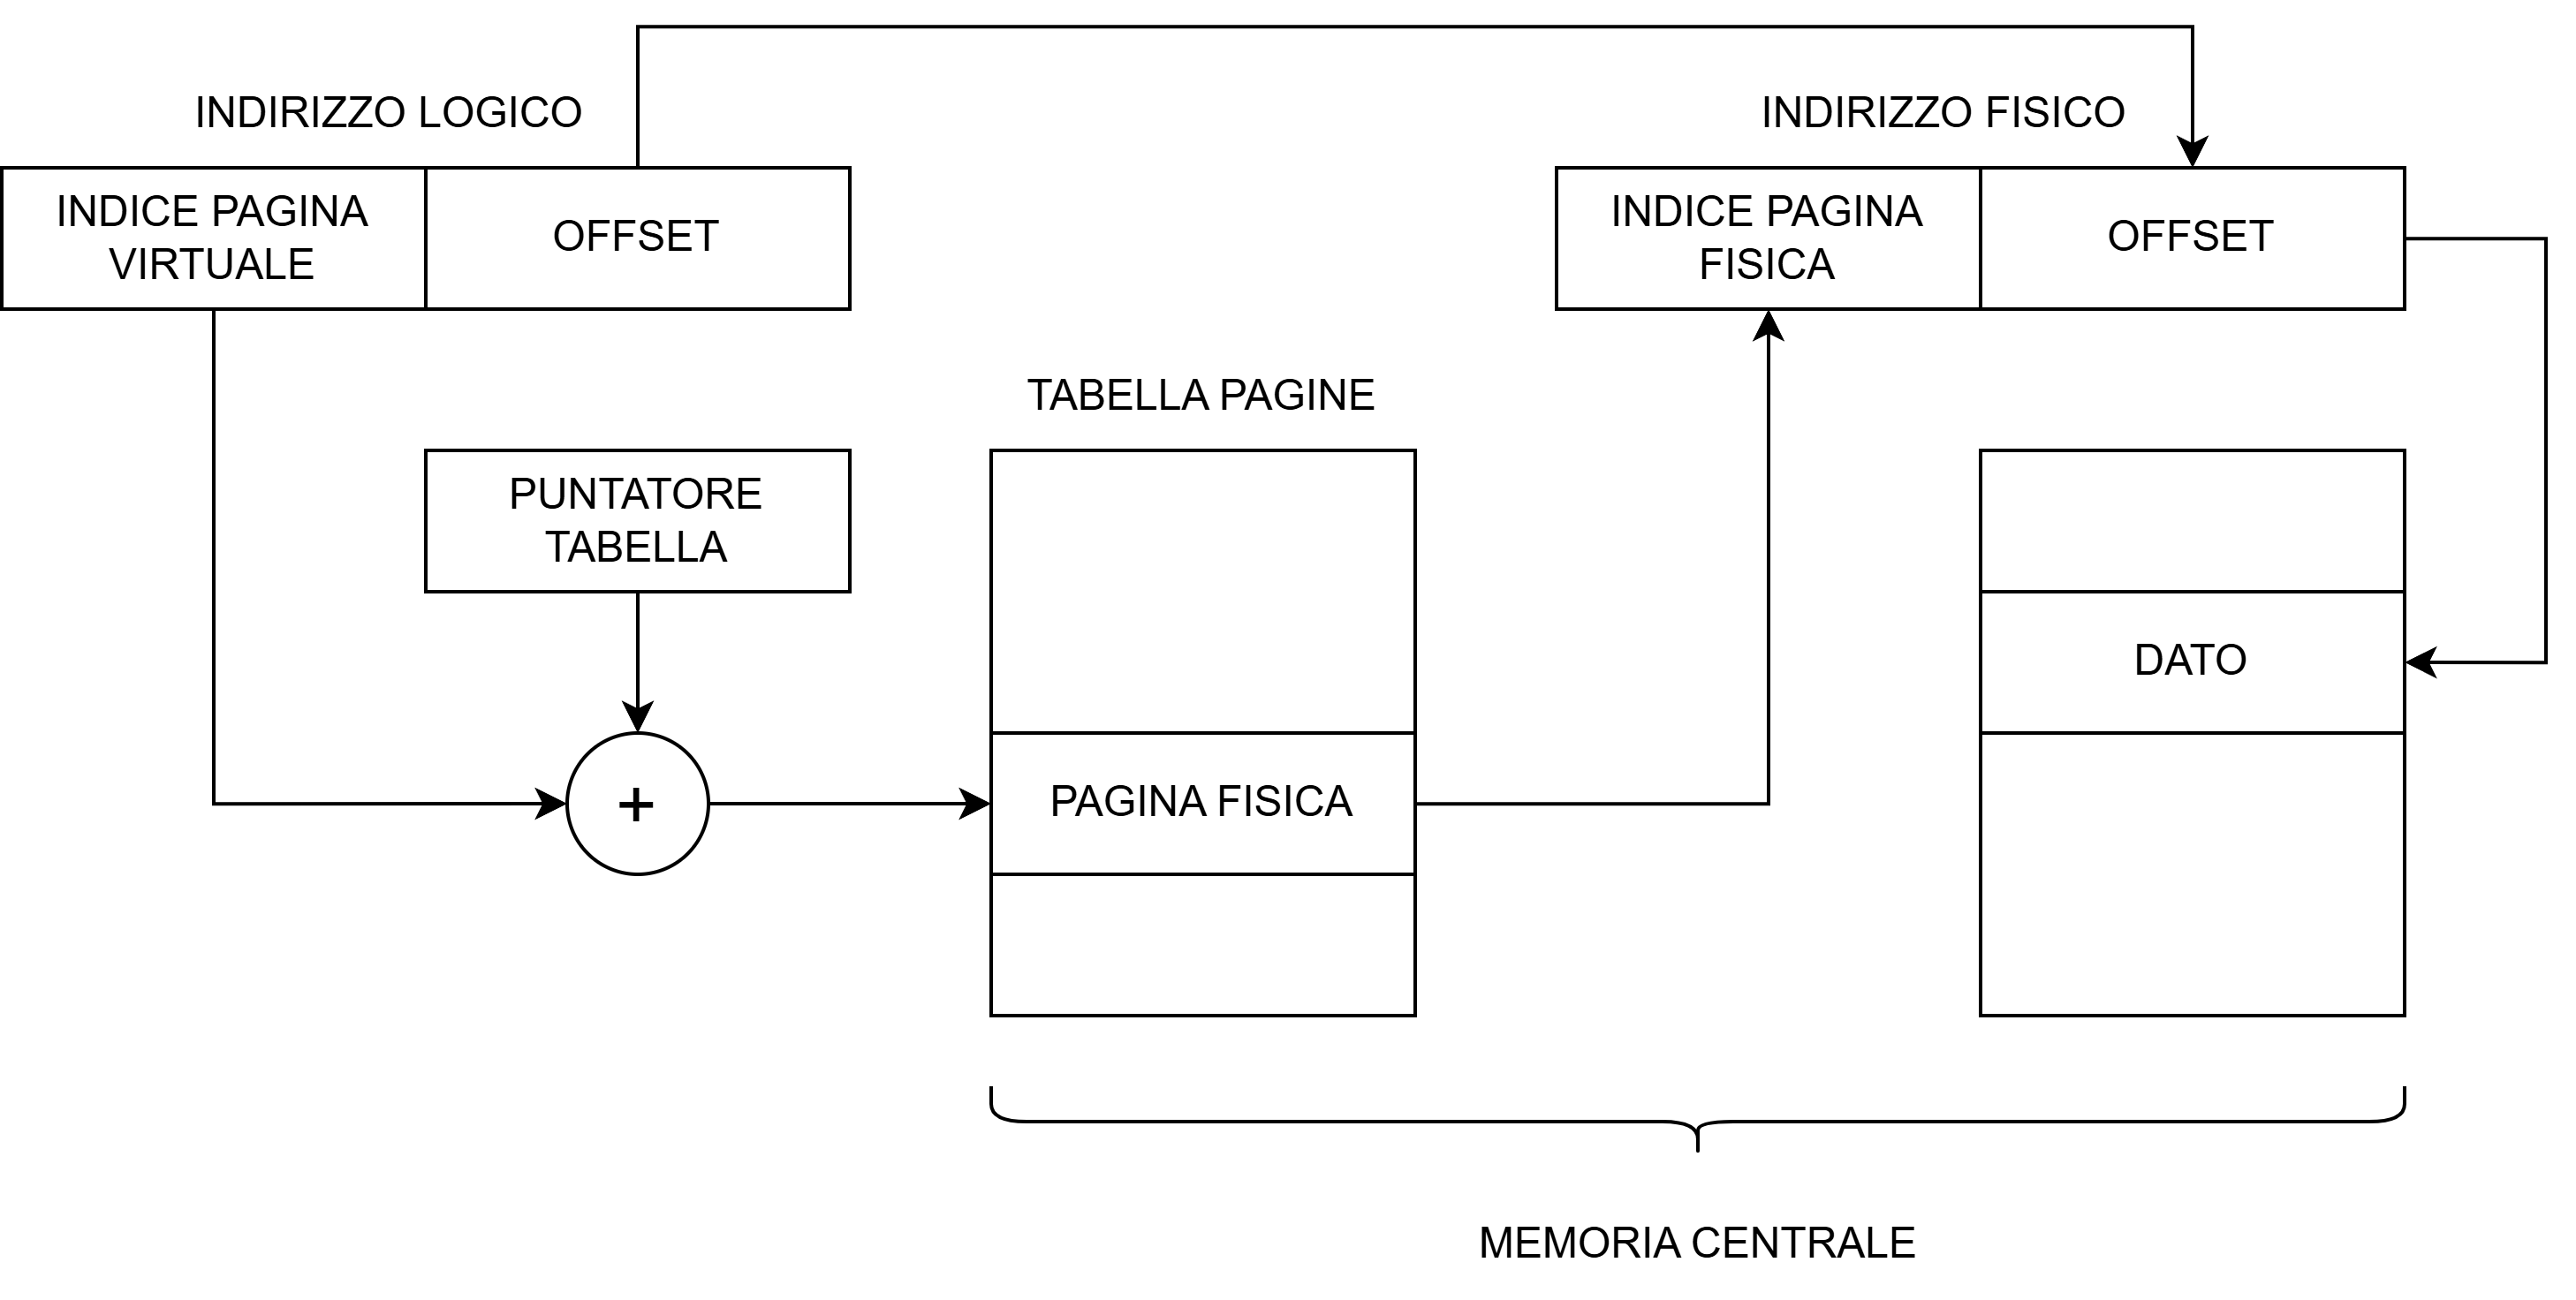
\includegraphics[width=0.65\linewidth]{img/traduzione.png}
    \caption{Processo di traduzione da indirizzo logico a fisico.}
    \label{fig:traduzione}
\end{figure}

Se durante il secondo passaggio la tabella delle pagine non trova alcuna corrispondenza, viene generata un'eccezione di tipo \textit{page fault} in seguito gestita dal sistema operativo, che ha il compito di attivare il driver che permette di leggere i dati dalla memoria di massa e scriverli in quella principale, aggiornando infine la tabella. In realtà, come anche anticipato durante la discussione degli elementi fondamentali delle memorie virtuali, esiste un importante componente noto come TLB che agisce da memoria cache per il processo di traduzione. Prima di procedere con la traduzione dell'indirizzo logico, la MMU consulta la TLB: se trova una corrispondenza, restituisce subito l'indirizzo base della pagina fisica; altrimenti, procede normalmente con il processo descritto in precedenza.
\\
\\
Un meccanismo di traduzione leggermente più avanzato consente di verificare se un certo dato è presente nella cache direttamente a partire dall'indirizzo logico, rimandando il calcolo dell'indirizzo fisico e addirittura evitando (quando possibile) il passaggio per il TLB. Per poter fare ciò, è necessario utilizzare come chiave dei blocchi in cache direttamente la parte di indice della pagina dell'indirizzo fisico, che in generale ha una dimensione maggiore essendo il numero di pagine maggiore del numero di blocchi. Con un tale approccio, si verificherebbe una complicazione in corrispondenza dei cache miss, poiché solo a seguito di questi si procederebbe alla traduzione dell'indirizzo. Per risolvere il problema, il componente di traduzione calcola preventivamente in parallelo l'indirizzo fisico, in modo tale che se il dato non è in cache non ci sono ulteriori sprechi di tempo per la traduzione. Tale sistema è noto come \textbf{virtual cache}. Notiamo come questo differisca dalla semplice traduzione spiegata in precedenza, che è un modello seriale, poiché passa sequenzialmente da indirizzo logico a fisico. Le cache virtuali non sempre sono utilizzate, in quanto complicano notevolmente il progetto delle memorie di primo e secondo livello.


\subsection{Cache e Memoria Virtuale}
In conclusione, cerchiamo di puntualizzare alcuni concetti generali che riguardano i sistemi che dispongono sia di memorie cache sia di meccanismi hardware e software per la gestione della memoria virtuale.
Il rapporto tra memoria virtuale e cache può in generale essere descritto tramite la seguente tabella [\ref{tab:cases_cache}].
\begin{table}[!h]
\centering
\begin{tabular}{|l|l|c|}
\hline
\textbf{Cache} & \textbf{Memoria Virtuale} & \textbf{Possibile?} \\
\hline
Miss & Page Fault & Sì \\
\hline
Miss & Page Hit & Sì \\
\hline
Hit & Page Fault & No \\
\hline
Hit & Page Hit & Sì \\
\hline
\end{tabular}
\caption{Compatibilità tra tipi di cache e memoria virtuale}
\label{tab:cases_cache}
\end{table}

Questa vuole stabilire che un dato presente in cache deve necessariamente essere anche presente nella memoria virtuale, in quanto una pagina è in grado di contenere più blocchi. Per lo stesso motivo, il viceversa non vale, ovvero un dato presente nella memoria virtuale non per forza sarà anche nella cache. 
\\
\\
La prima osservazione è che i meccanismi di gestione della memoria virtuale consentono di determinare se e in quale posizione della memoria centrale è contenuto un dato o un'istruzione, mentre la cache è unicamente un sistema per velocizzare l'accesso a dati e istruzioni. Banalmente, ne deriva che se nel caso in cui il dato contenuto in una pagina non sa presente in memoria centrale, non potrà essere presente neanche nella cache. \MakeUppercase{è} bene notare, che dal punto di vista funzionale per il processore sia la presenza della cache che quella della memoria virtuale è del tutto trasparente, in quanto tali soluzioni architetturali sono in grado di garantire che ogni richiesta di accesso a un dato da parte del processore sia sistematicamente sempre eseguita, indipendentemente da dove questo è situato.
\\
\\
Vi sono notevoli similitudini tra il principio di funzionamento delle cache della memoria virtuale, in quanto entrambe sono basati sui principi di località e gerarchia. Tuttavia, le differenze tra le due sono molto profonde, e vanno oltre le sole differenze nei tempi di accesso. Innanzitutto, le dimensioni dei blocchi delle cache sono minori di quelle delle pagine, stanti le differenti dimensioni delle memorie in gioco. Ne consegue che la possibilità di non trovare un dato nella cache è molto più alta di quella di non trovare un dato in una pagina residente in memoria. Altra sostanziale differenza sta nel fatto che la gestione della memoria cache è sempre fatta totalmente in hardware per esigenze prestazionali. La gestione della memoria virtuali, invece, può avvenire secondo due modalità: operando su indirizzi fisici come fa la memoria centrale, oppure operando su indirizzi logici (virtual cache). Una cache che utilizza indirizzi fisici è in generale più lenta, perché prima deve essere eseguita un'operazione di traduzione per ottenere un corrispondente indirizzo logico, cosa che richiede del tempo, da aggiungere a quello richiesto dall'operazione di accesso della cache. Qualora invece l'indirizzo in ingresso alla cache sia virtuale, non è necessaria alcuna traduzione preventiva, rendendo il processo più veloce poiché l'operazione di traduzione avviene soltanto in caso di cache miss. Gli svantaggi di tale approccio sono una maggiore complessità nella gestione della allocazione dei dati nella cache. Ad esempio, nel caso di sistemi multitasking, due processi distinti potrebbero voler accedere a uno stesso indirizzo virtuale che poterebbe entrambi a indirizzare lo stesso dato in cache invece di dati distinti. Le soluzioni in questo caso sono due:
\begin{enumerate}
    \item L'uso di un unico spazio di memoria virtuale comune a tutti i processi del sistema. Questa soluzione che elimina alla base il problema è stata resa possibile dalla disponibilità nei processori più recenti di indirizzi a 64 bit.
    \item La possibilità di invalidare la cache e rinnovarla completamente (cache flushing) a seguito di un task switching. In questo modo, i dati nella cache sarebbero riferibili a un solo processo, ma ciò influisce negativamente sulle prestazioni.
\end{enumerate}